\documentclass[12pt]{report}
\usepackage{amssymb}
\usepackage{multicol}
\usepackage{graphicx}
\usepackage{subfigure}
\usepackage{verbatim}
\usepackage[letterpaper,left=1cm,right=2cm, top=1.5cm,
bottom=1.3cm,head=0cm,foot=1cm]{geometry}

\parindent=0in

\newcommand{ \probDir}[1]{{ \bf\small #1 \mbox{  }}}

\newcommand{ \breakList}{\setcounter{saveenum}{\value{enumi}} \end{enumerate}}
\newcommand{ \contList}{\begin{enumerate} \setcounter{enumi}{\value{saveenum}}}


\newcounter{saveenum}

%%%%%%%%%%%%%%%%%%%%%%%%%%%%%%%%%%%%%%%%%
\begin{document}

{\bf{Honors Physics} \hfill {Algebra Worksheet 2} \hfill {Mr. Kelley}} \\ \\
%%%%%%%%%%
\probDir{Solve the following equations for $x$:} \\
%%%%%%%%%%
\begin{multicols}{3}
\begin{enumerate}
\item $\frac{2x}{5} =  z$
\item $\frac{5}{2x} =  z$
\item $4x - 3y = 7y$
\item $7z - 2zx = 10zy$
\item $4x^{2} - 12x = 44$
\item $A = 4\pi x^2$
\item $21 = \frac{7x}{5y}$
\item $\frac{x}{8} = \frac{4y}{7x}$
\item $\frac{2t}{5x} + \frac{1}{10x} = 3t$
\item $F=k\frac{ab}{x^2}$
\item $8tx + 8t = 12x$
\item $\frac{1}{x} = \frac{1}{y} + \frac{1}{z}$
\breakList
\end{multicols}
%%%%%%%%%%
\probDir{Write $x$ as a function of $t$:}
%%%%%%%%%%
\begin{multicols}{2}
\contList
\item $5t + 21x = 15$
\item $t^2 - 2xt = t$
\item $12xt = 4t^2 - 4t+2x$
\item $\frac{x}{t} - v_{\circ}= \frac{1}{2}at$
\breakList
\end{multicols}

\contList
\item \probDir{What is the value of $x(4)$ in the following figures?}

\begin{figure}[h]
\centering
\subfigure[]{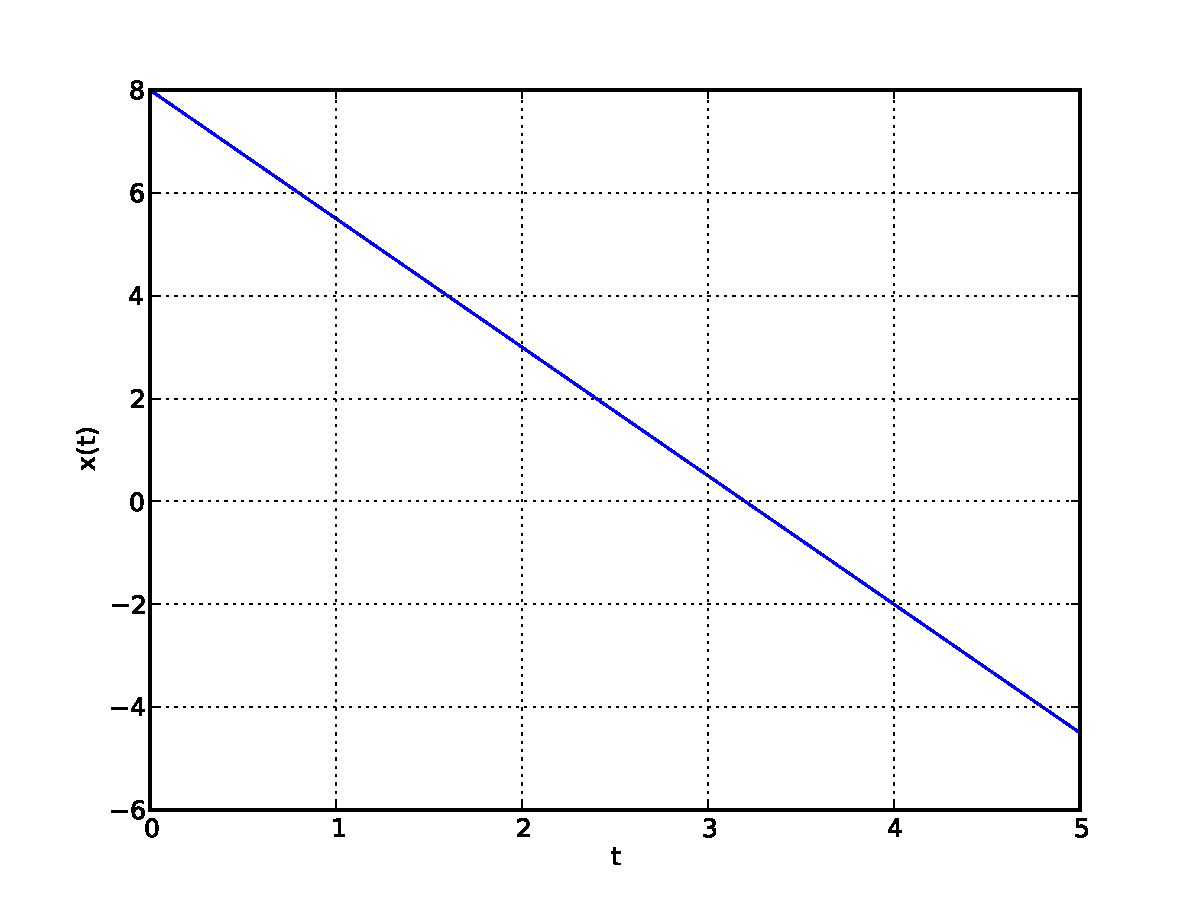
\includegraphics[scale = .45]{fig20.pdf}}
\subfigure[]{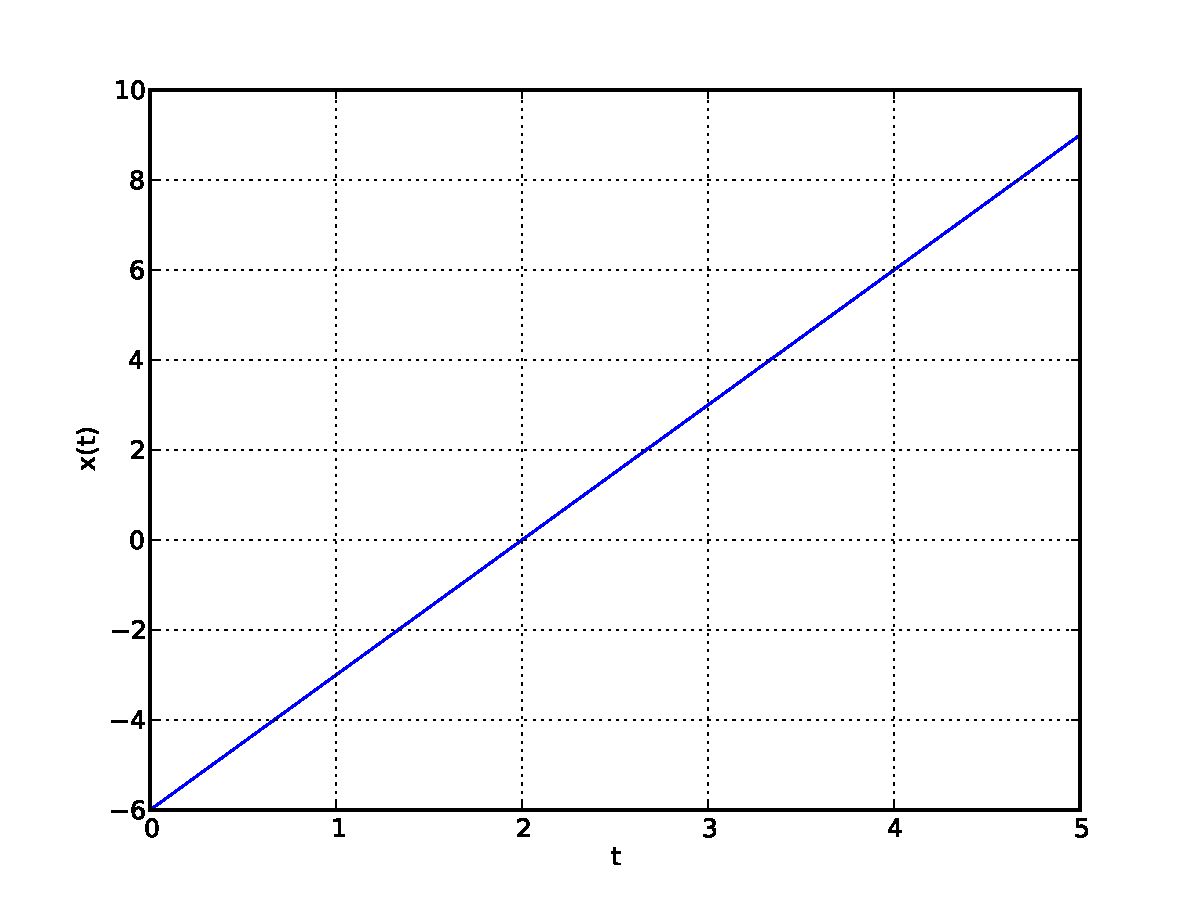
\includegraphics[scale = .45]{fig21.pdf}}
\subfigure[]{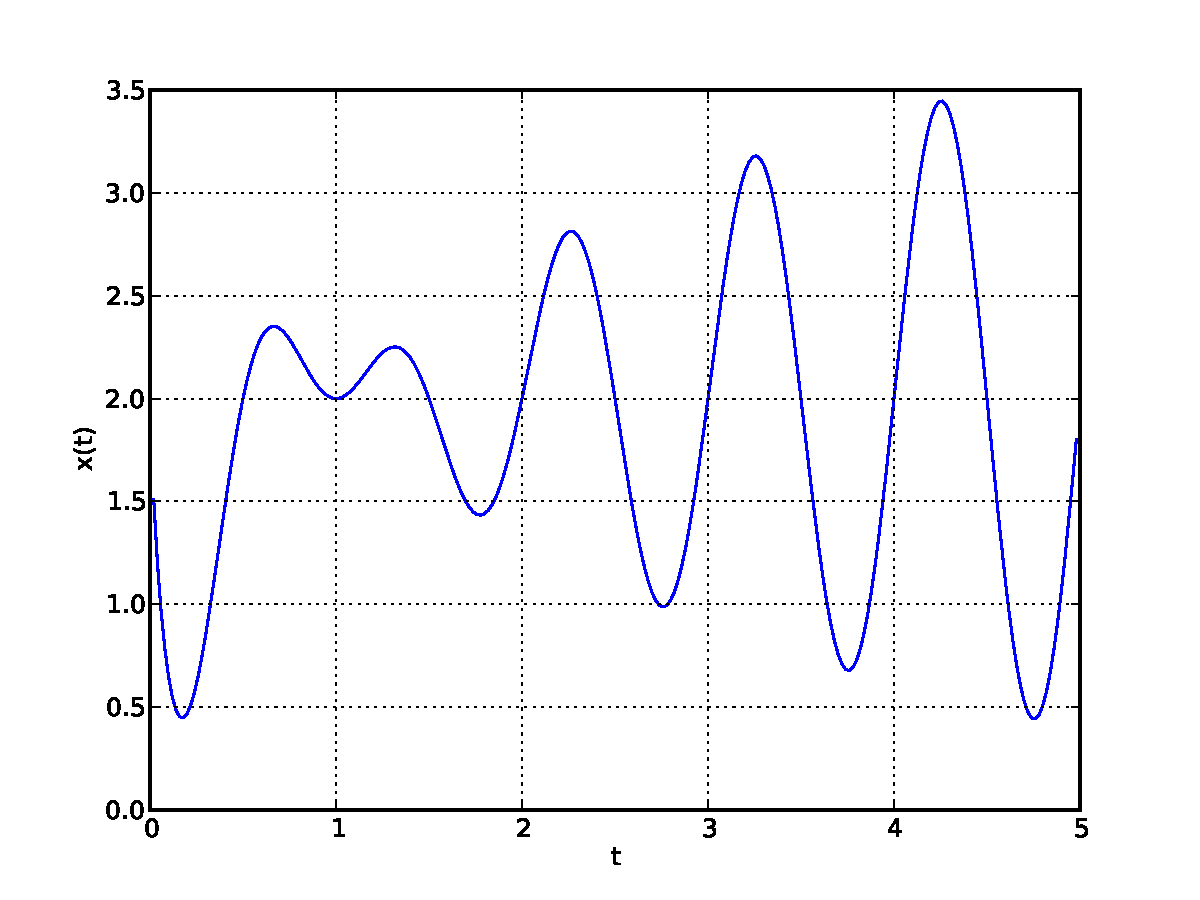
\includegraphics[scale = .45]{fig22.pdf}}
\subfigure[]{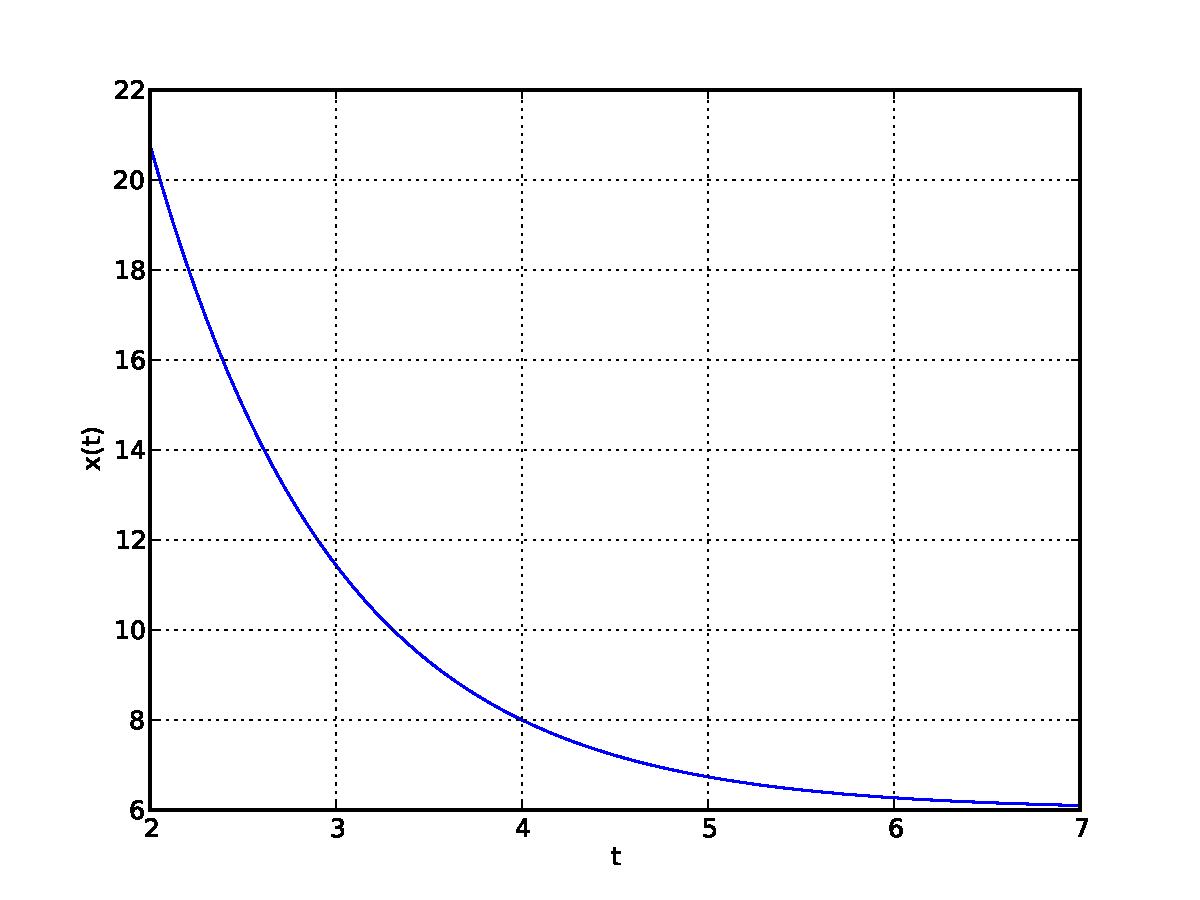
\includegraphics[scale = .45]{fig23.pdf}}
\setcounter{subfigure}{0}
\end{figure}

\pagebreak
%%%%%%%%%%%%%%

\item What is $x(0)$ in problem 13.
\item What is $x(1)$ in problem 14.
\item What is $x(-1)$ in problem 15.
\item What is $x(0)$ in problem 16.

\probDir{Use the figure to complete the following problems}

\begin{figure}[h]
\centering
\subfigure{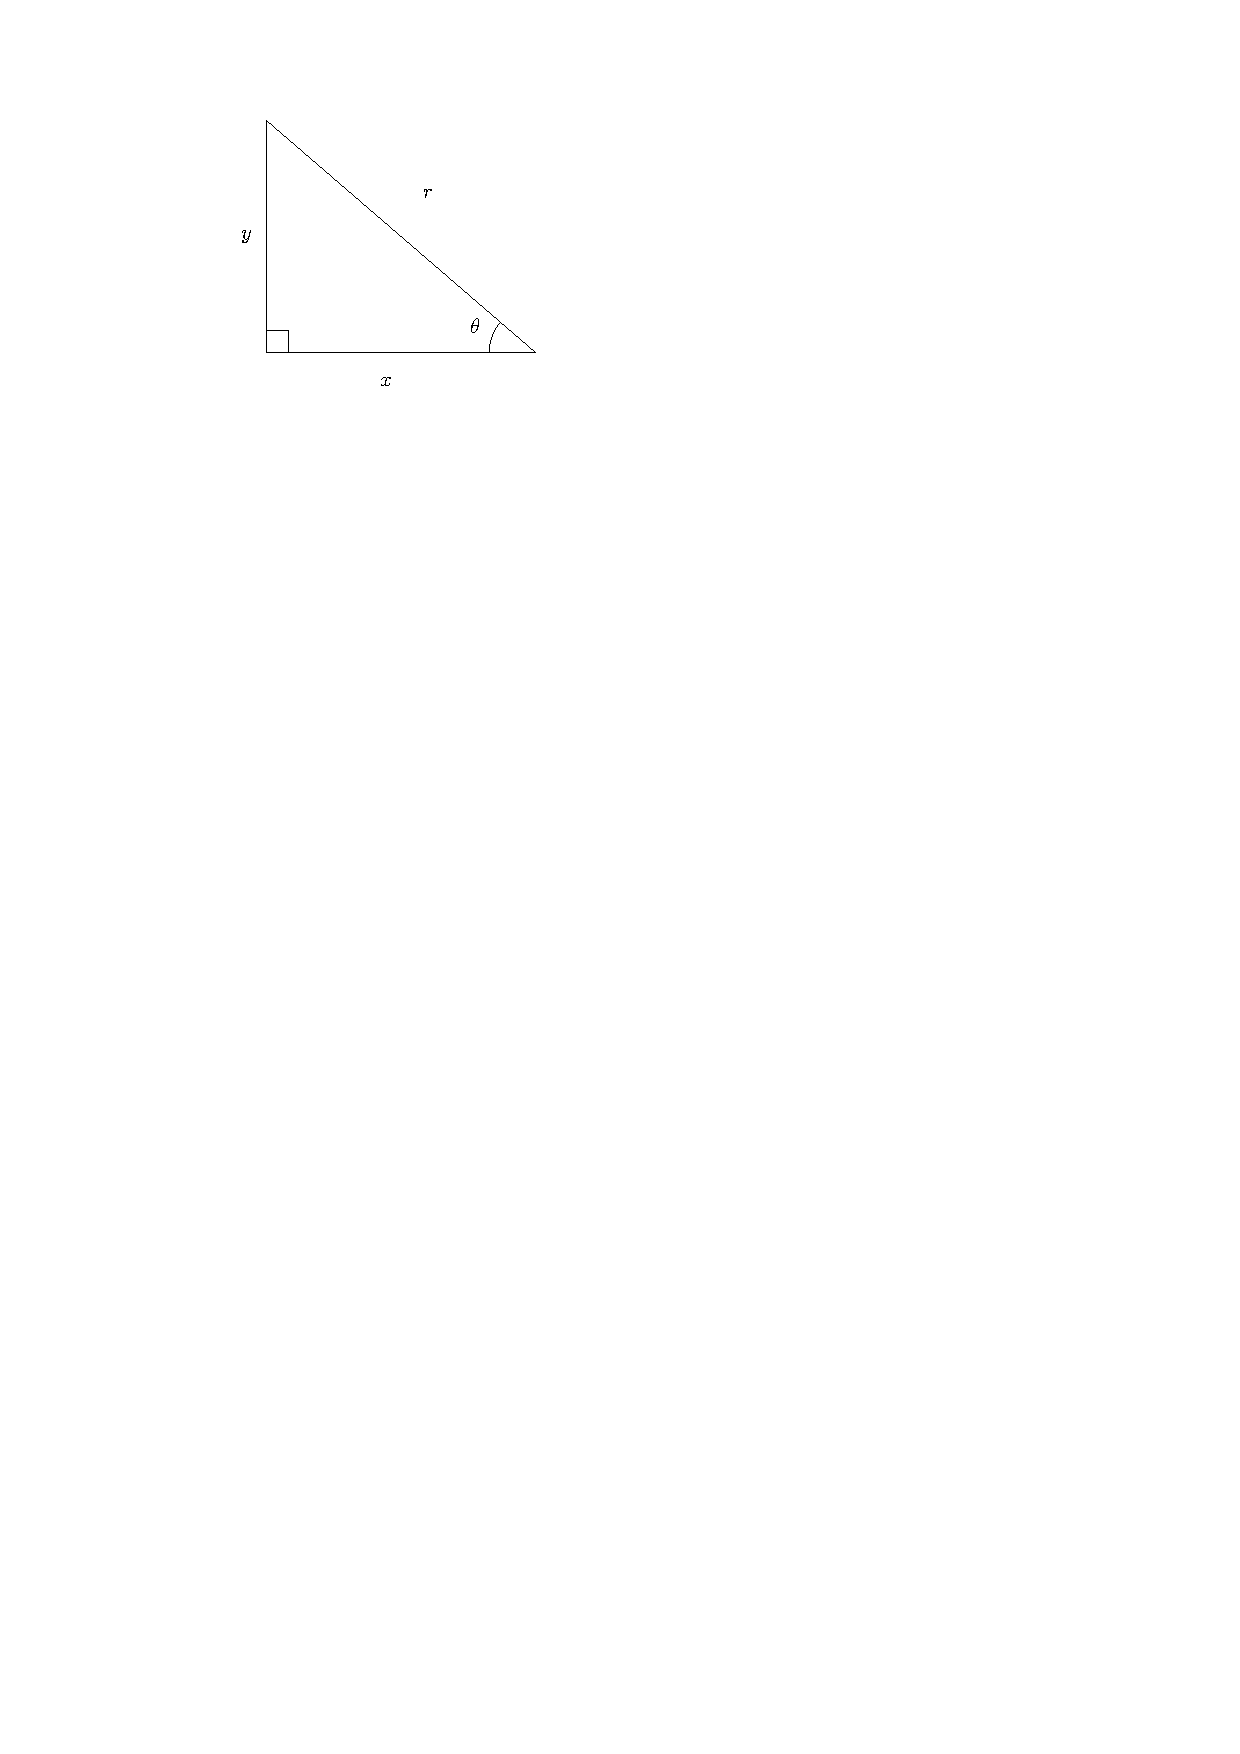
\includegraphics[scale = 1]{rightTriangle.pdf}}
\setcounter{subfigure}{0}
\end{figure}

\begin{multicols}{2}
\item $x = 5$, $y = 7$, $r=$?, $\theta = $?
\item $x = 1$, $y = 2$, $r=$?, $\theta = $?
\item $r=32$, $\theta = 45^\circ$, $x = $?, $y = $?
\item $r=100$, $\theta = 66^\circ$, $x = $?, $y = $?
\item $r=1$, $\theta = 20^\circ$, $x = $?, $y = $?
\item $r=44$, $\theta = 79^\circ$, $x = $?, $y = $?
\end{multicols}

\item \probDir{Find $a$ and $b$ in the following figures.}

\begin{figure}[h]
\centering
\subfigure[]{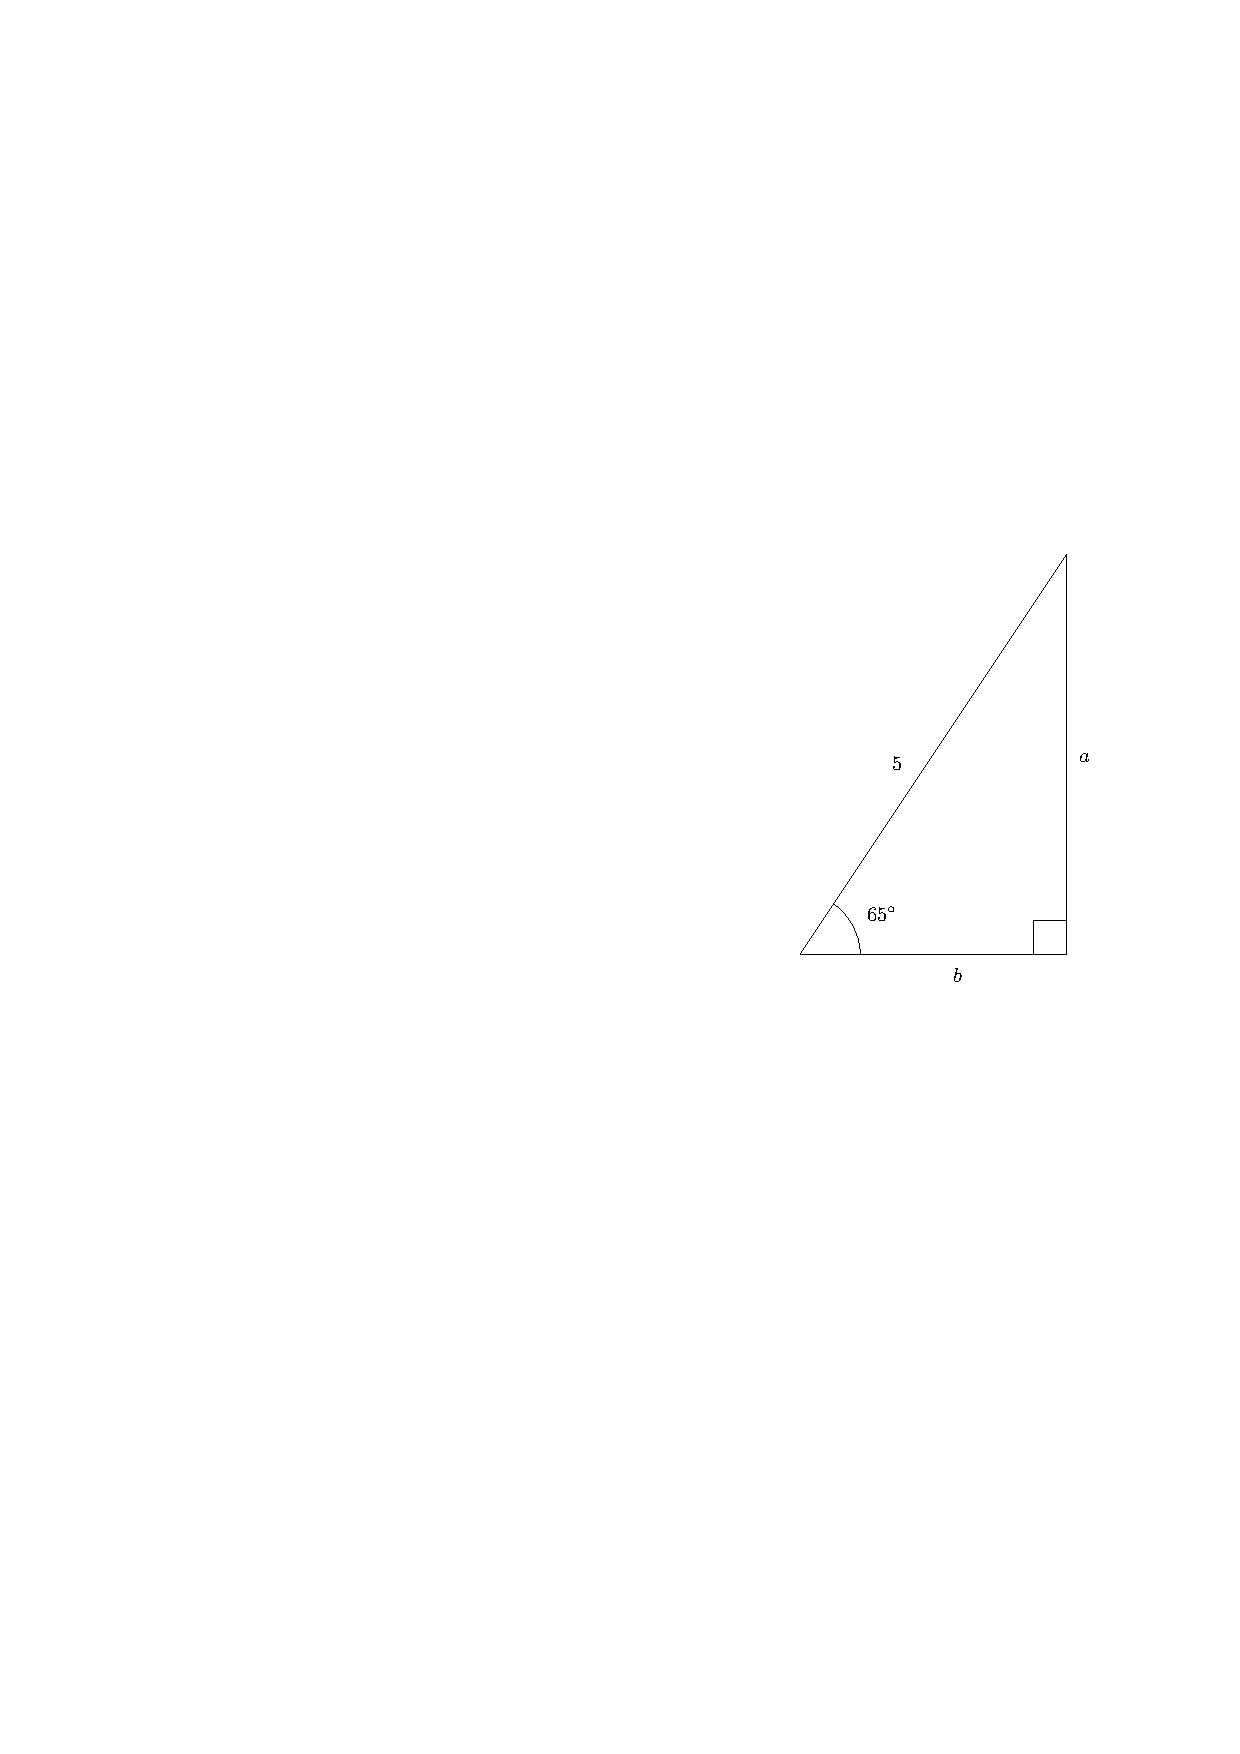
\includegraphics[scale = .8]{rt3.pdf}}
\subfigure[]{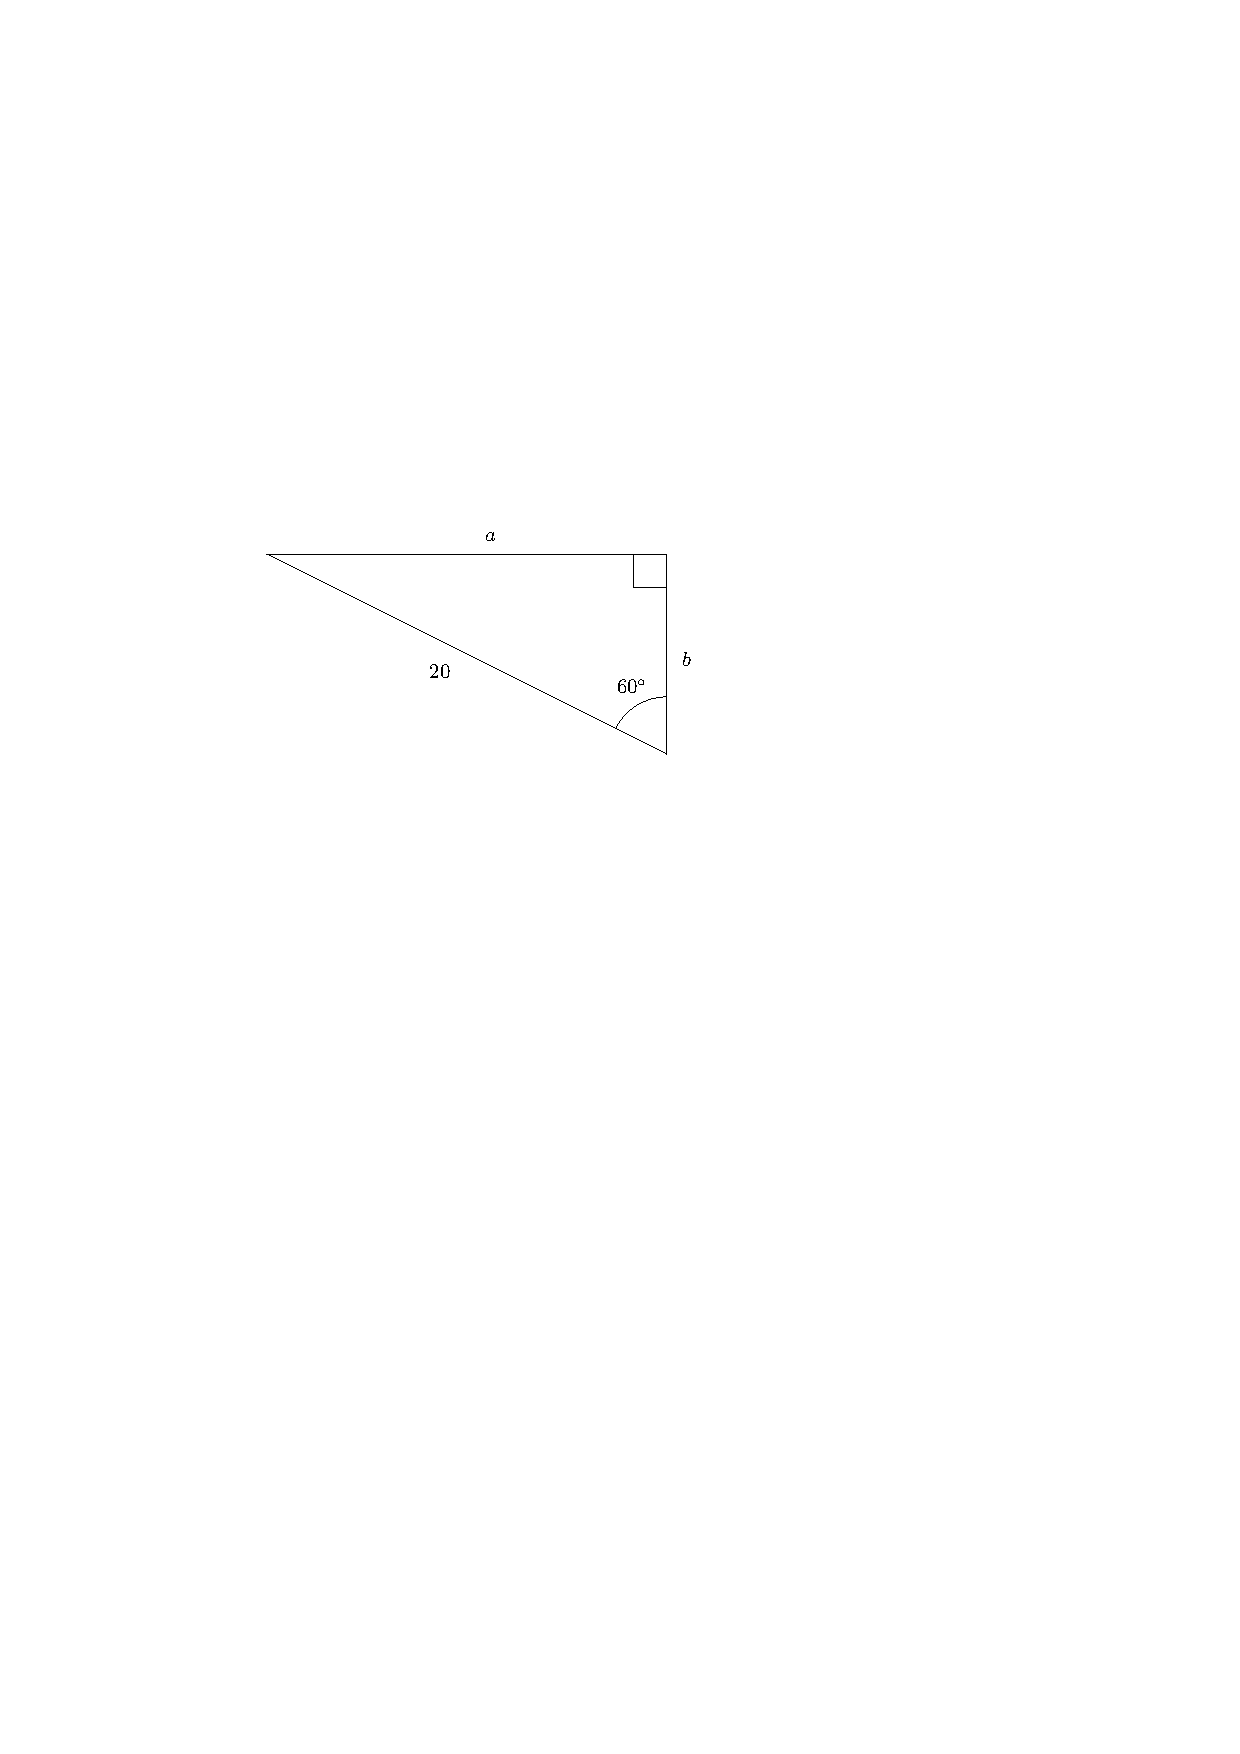
\includegraphics[scale = .8]{rt2.pdf}}
\subfigure[]{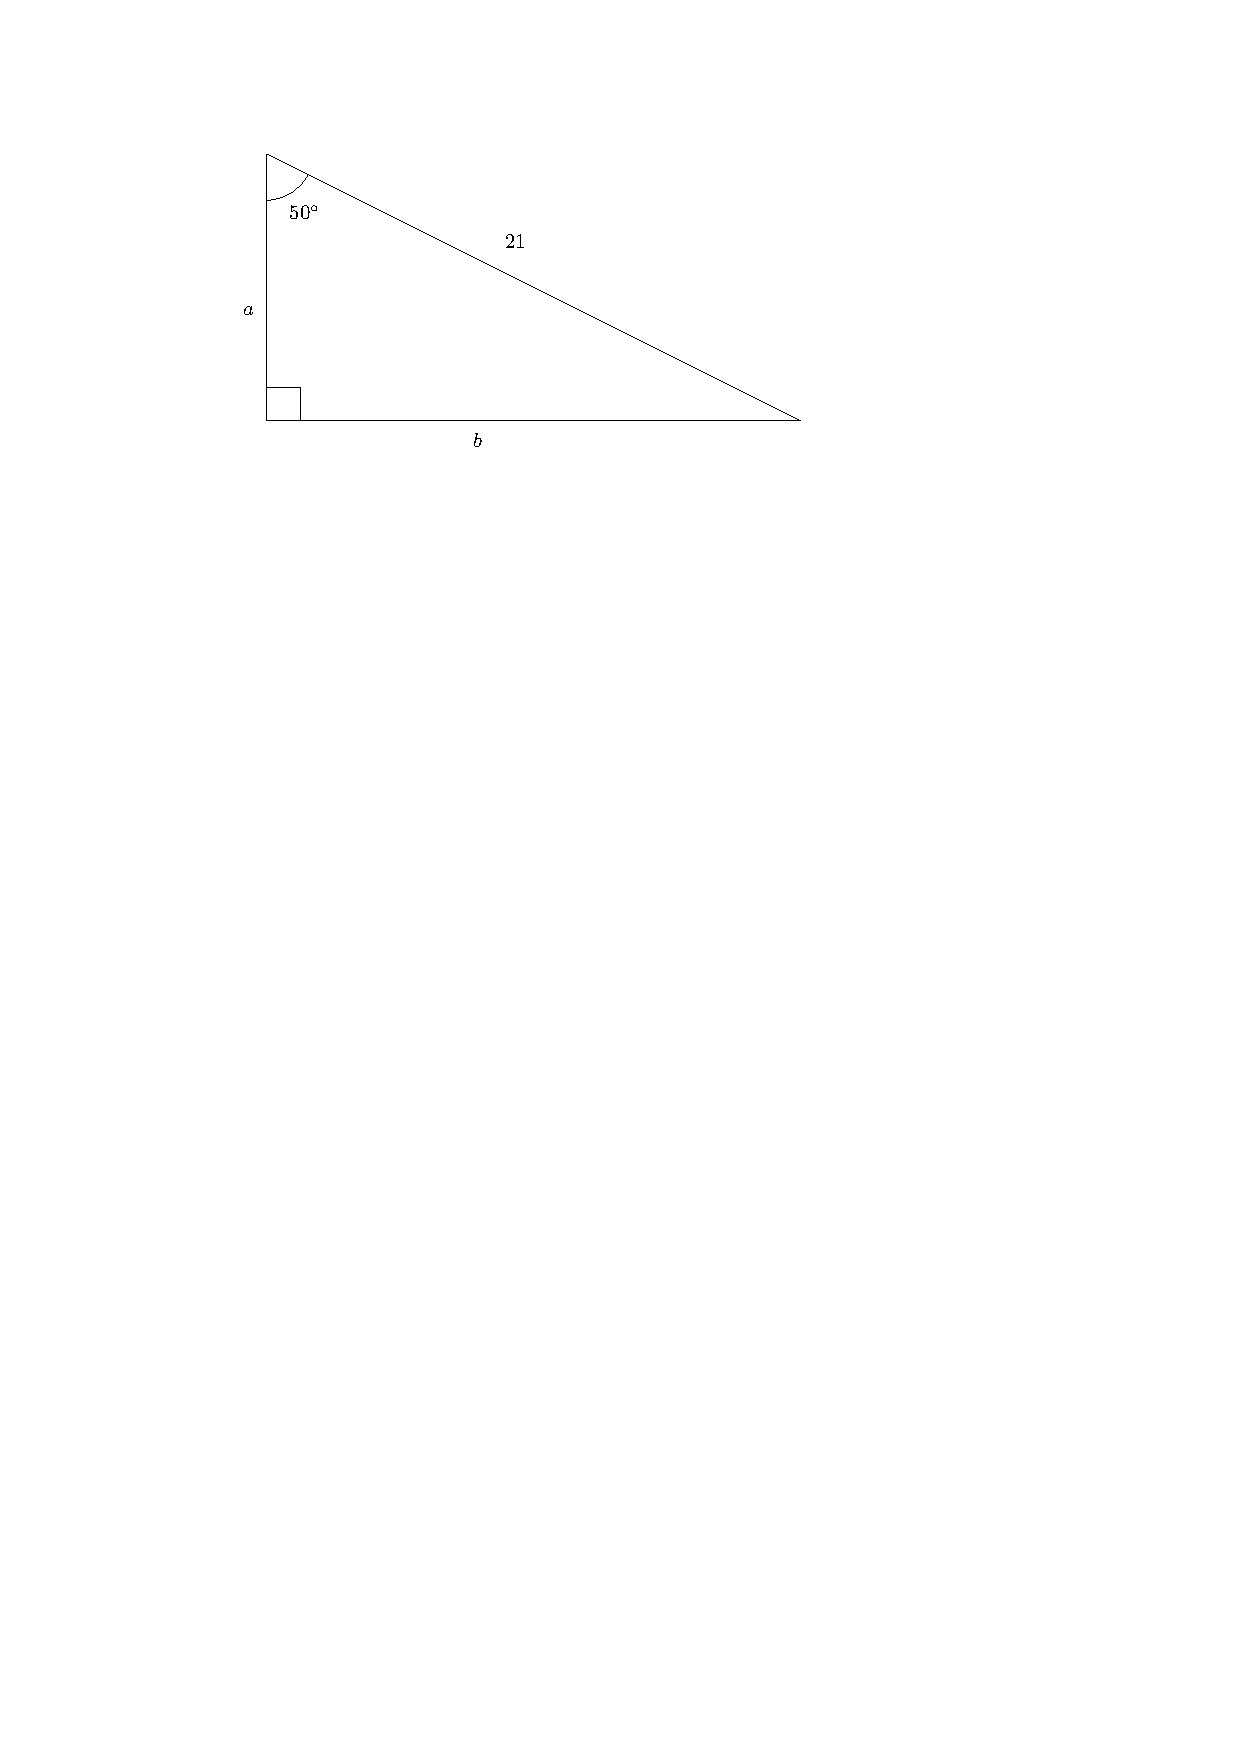
\includegraphics[scale = .8]{rt1.pdf}}
\subfigure[]{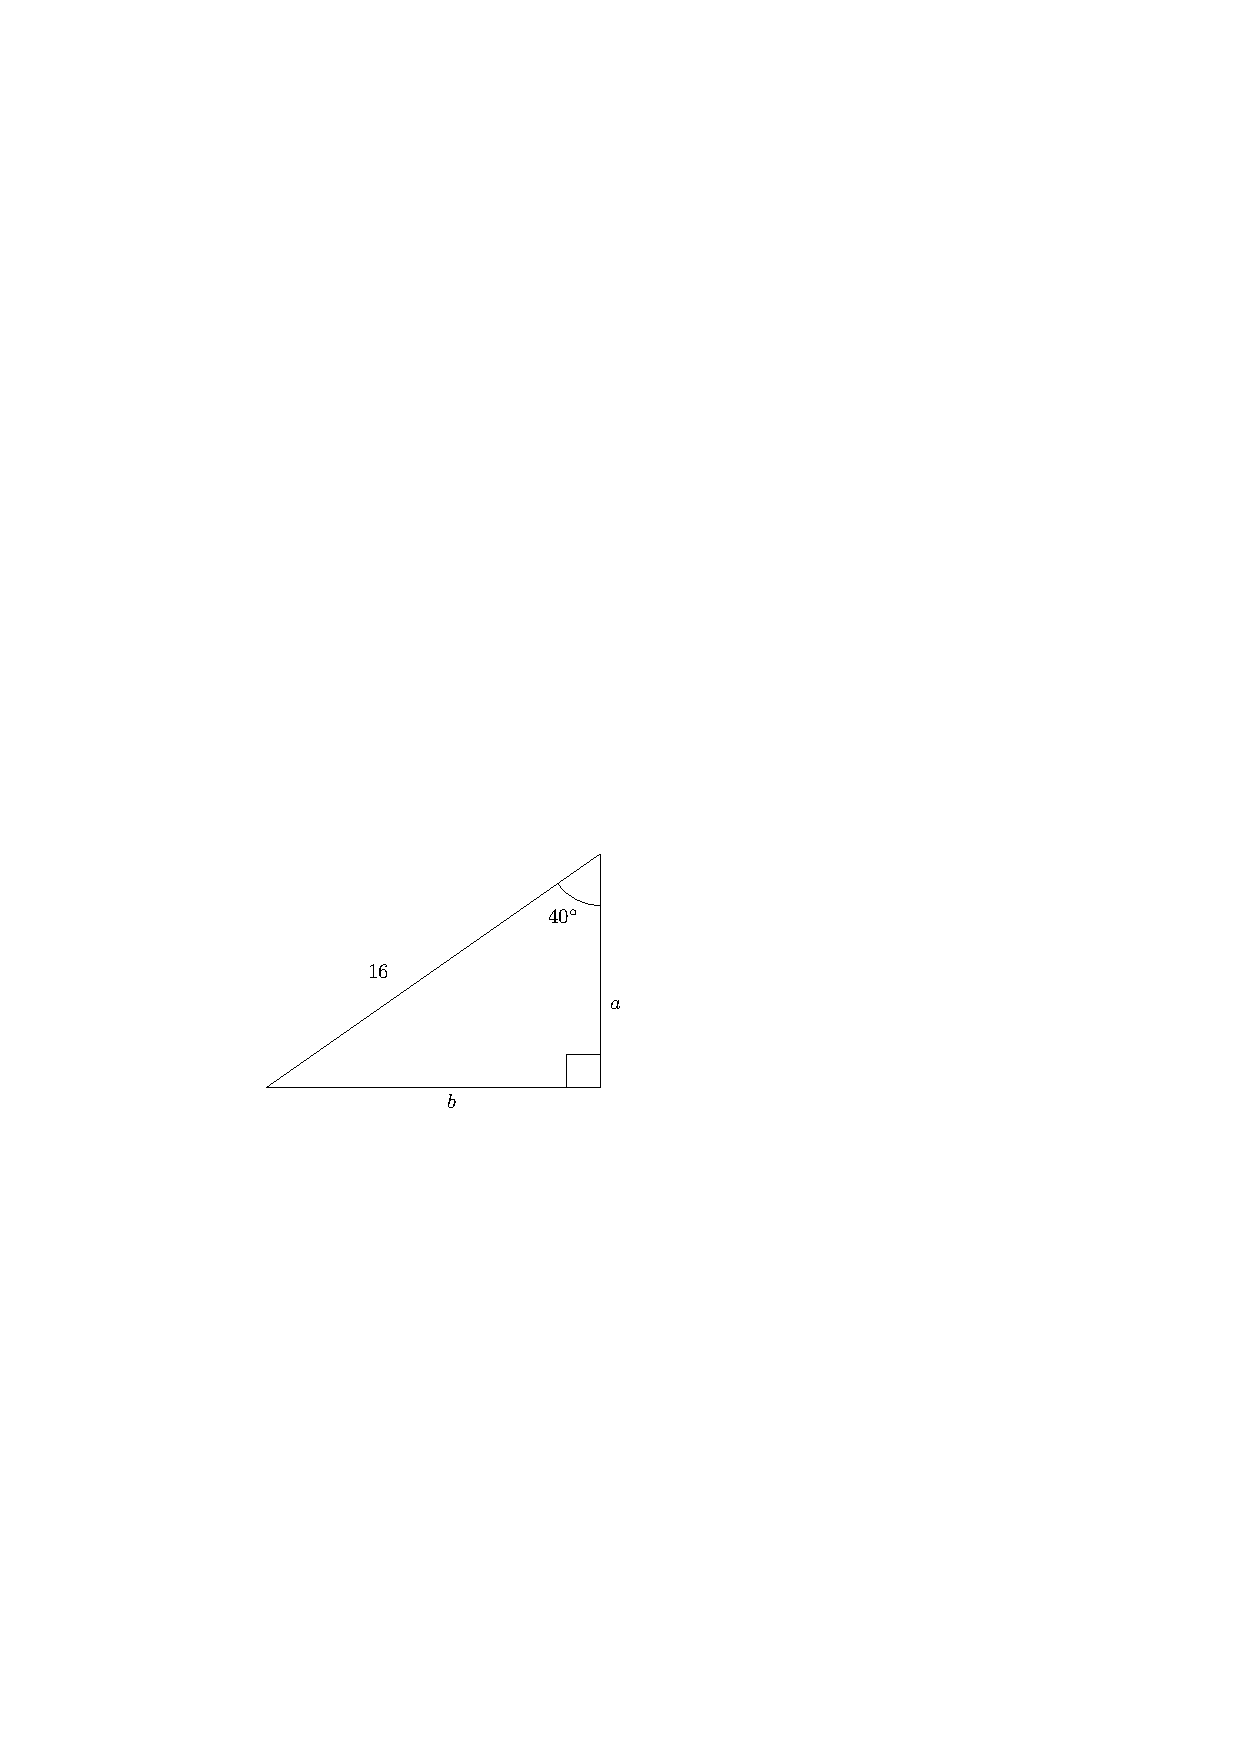
\includegraphics[scale = .8]{rt4.pdf}}
\setcounter{subfigure}{0}
\end{figure}


\end{enumerate}

\end{document}